\chapter{Data and Training Pipeline}

\section*{Why This Matters}

Data quality and pipeline efficiency determine training success more than architectural choices. A well-designed model trained on poor data underperforms a simpler model trained on high-quality data. Understanding data requirements, preprocessing strategies, and pipeline optimization is essential for accurate project scoping, timeline estimation, and resource allocation.

The data pipeline—from raw data acquisition through preprocessing, augmentation, and batching—typically consumes 40-60\% of total project time. Pipeline bottlenecks directly impact training efficiency: a GPU waiting for data wastes expensive compute resources. Data quality issues discovered late in training waste weeks of work and thousands of dollars in compute costs.

This chapter examines data pipeline architecture from an engineering perspective, focusing on quality requirements, preprocessing strategies, pipeline optimization, and the trade-offs that determine project success and cost efficiency.

\section{Data Requirements and Quality}

\subsection{Training Data Scale}

Transformer models require substantial training data to achieve production-quality performance. The relationship between model size and data requirements follows empirical scaling laws that inform project planning and data acquisition strategies. Small models with fewer than 100 million parameters typically require 1-10 billion tokens minimum for adequate training. Medium models ranging from 100 million to 1 billion parameters need 10-100 billion tokens. Large models exceeding 1 billion parameters demand 100 billion to 1 trillion tokens or more.

For BERT-base with its 110 million parameters, the original training used 3.3 billion tokens from Wikipedia and BookCorpus. GPT-3, with 175 billion parameters, trained on 300 billion tokens. These scales represent minimum viable training data—more data generally improves performance up to a point, though with diminishing returns.

The economic implication becomes clear when considering data acquisition costs. At typical rates of \$0.01-0.10 per labeled example, collecting 100,000 labeled examples costs \$1,000-10,000. For large-scale pretraining, web scraping, cleaning, and deduplication infrastructure can cost \$50,000-500,000 to build and operate. These data costs often exceed training compute costs, making data strategy a primary economic consideration.


\subsection{Data Quality Dimensions}

Data quality encompasses multiple dimensions, each with specific implications for model performance and project costs. Accuracy—the correctness of labels and annotations—directly determines the model's quality ceiling. A model trained on 90\% accurate labels cannot reliably exceed 90\% accuracy, making label validation and inter-annotator agreement measurement essential quality controls. The relationship is direct and unforgiving: label quality caps model quality.

Completeness refers to coverage of the target distribution. Training data must represent the full range of inputs the model will encounter in production. Gaps in coverage lead to poor performance on underrepresented cases, often requiring domain-specific data collection beyond public datasets. For enterprise applications, this frequently means investing in custom data collection that captures organization-specific terminology, workflows, and edge cases.

Consistency ensures uniform annotation standards across the dataset. Inconsistent labeling introduces noise that degrades model performance and increases training time. Annotation guidelines, annotator training, and quality audits maintain consistency. The cost of inconsistency manifests as longer training times and lower final performance—both expensive outcomes.

For domains with evolving language or concepts—news, social media, technical documentation—freshness matters significantly. Stale training data degrades production performance as the gap between training distribution and production distribution widens. This necessitates continuous data collection and periodic retraining, adding ongoing operational costs to the initial training investment.

Representativeness measures the distribution match between training and production data. Distribution shift, when production data differs systematically from training data, is a primary cause of production failures. Measuring and minimizing this shift requires careful sampling strategies during data collection and ongoing monitoring in production. The challenge intensifies when production distribution evolves over time, requiring adaptive data collection strategies.

\subsection{Data Quality Economics}

Data quality improvements follow diminishing returns that shape investment decisions. Moving from 80\% to 90\% label accuracy might cost \$10,000 in additional annotation effort. Moving from 90\% to 95\% might cost \$50,000 as annotators must resolve increasingly subtle cases. Moving from 95\% to 99\% might cost \$200,000 as only the most difficult examples remain, requiring expert annotators and extensive quality control.

The optimization question centers on justifiable cost. For high-stakes applications like medical diagnosis or legal analysis, 99\% accuracy requirements justify substantial quality investment. The cost of errors—misdiagnosis, legal liability—far exceeds annotation costs. For lower-stakes applications like content recommendations or search ranking, 90-95\% accuracy often provides acceptable performance at much lower cost. The business impact of marginal accuracy improvements doesn't justify the exponentially increasing annotation costs.

\begin{figure}[htbp]
\centering
\includegraphics[width=0.9\textwidth]{chapters/diagrams/chapter08_quality_cost_i9j0k1l2.pdf}
\caption{Data quality versus cost curve showing exponential cost increase for marginal accuracy improvements. The 80-92\% range represents cost-effective quality for most applications, while 95-99\% accuracy is justified only for high-stakes domains where error costs exceed annotation costs.}
\label{fig:quality_cost}
\end{figure}


\begin{tcolorbox}[colback=blue!5!white,colframe=blue!75!black,title=\textbf{IN PRACTICE: Data Quality ROI}]

\textbf{Scenario}: Customer support chatbot for e-commerce company

\textbf{Standard Quality Approach} (90\% label accuracy): Data collection of 50,000 examples at \$0.50 per example costs \$25,000. The resulting model achieves 87\% accuracy, leading to 78\% customer satisfaction and 40\% support cost reduction.

\textbf{High Quality Approach} (95\% label accuracy): The same 50,000 examples cost \$1.50 each due to additional validation requirements, totaling \$75,000. Additional validation processes add \$15,000, bringing total investment to \$90,000. The resulting model achieves 91\% accuracy, leading to 85\% customer satisfaction and 55\% support cost reduction.

\textbf{Analysis}: The additional \$65,000 investment yields 15\% additional support cost reduction. With \$2 million in annual support costs, this translates to \$300,000 in additional annual savings. The payback period is 2.6 months, making the high-quality approach clearly justified by substantial operational savings.

\end{tcolorbox}

\section{Data Preprocessing Pipeline}

\subsection{Pipeline Architecture}

The data preprocessing pipeline transforms raw data into model-ready format through multiple stages. Each stage presents specific engineering trade-offs between quality, throughput, and resource consumption. Understanding these stages and their bottlenecks enables effective pipeline design and optimization.

Data ingestion forms the first stage, collecting raw data from various sources including databases, APIs, and files. This stage standardizes formats—converting diverse inputs into consistent JSON, CSV, or Parquet representations—and performs initial validation and filtering. Typical throughput ranges from 10-100 GB per hour, primarily limited by network bandwidth and source system performance rather than processing capacity.

Cleaning and filtering constitute the most computationally intensive stage. Duplicate removal requires comparing documents for exact and near-duplicate matches, a quadratic operation that becomes expensive at scale. Quality filtering examines length, language, and content type, rejecting documents that don't meet criteria. Noise removal strips HTML tags, special characters, and formatting artifacts. This stage typically achieves 1-10 GB per hour throughput, constrained by CPU processing rather than I/O.

Tokenization segments text into tokens—subword units that form the model's vocabulary. This process maps each token to a unique integer ID and inserts special tokens like [CLS], [SEP], and [PAD] that provide structural information to the model. Tokenizer complexity varies significantly: simple whitespace tokenization processes 50 GB per hour, while sophisticated subword tokenizers like SentencePiece or WordPiece achieve 5-10 GB per hour due to their algorithmic complexity.


Sequence construction chunks tokenized text into fixed-length sequences suitable for model input. This involves padding shorter sequences to target length, truncating longer sequences, and generating attention masks that indicate which positions contain real tokens versus padding. This stage operates primarily on memory, achieving 10-100 GB per hour throughput.

Batching and shuffling group sequences into training batches and randomize their order for training stability. Random shuffling prevents the model from learning spurious patterns based on data ordering. Batch serialization prepares data for efficient loading during training. This stage is I/O bound, achieving 50-500 GB per hour depending on storage performance.

\subsection{Pipeline Bottlenecks}

Pipeline throughput determines training efficiency in a direct and costly way. A GPU capable of processing 1,000 sequences per second achieves only 100 sequences per second if data loading provides only 100 sequences per second. The GPU sits idle 90\% of the time, wasting expensive compute resources. Identifying and addressing bottlenecks is essential for cost-effective training.

Disk I/O frequently limits throughput when reading data from storage. SSDs provide 500-3,000 MB per second while HDDs provide only 100-200 MB per second. For large datasets exceeding 100 GB, disk I/O often becomes the limiting factor. The solution involves parallel loading from multiple drives, in-memory caching of frequently accessed data, or migration to faster storage. The cost-benefit calculation depends on training frequency: for one-time training, slow storage suffices; for continuous training, fast storage pays for itself quickly.

CPU processing limits throughput during tokenization, filtering, and transformation. Single-threaded processing restricts throughput to 1-10 GB per hour regardless of disk speed. Multiprocessing distributes work across CPU cores, vectorized operations leverage SIMD instructions, and compiled implementations replace interpreted Python code. These optimizations typically provide 4-8× speedup, often sufficient to eliminate CPU bottlenecks.

Memory bandwidth constrains data movement between CPU and GPU. PCIe 3.0 provides approximately 12 GB per second while PCIe 4.0 provides approximately 24 GB per second. For small batches or frequent transfers, memory bandwidth becomes the limiting factor. Larger batches amortize transfer overhead, prefetching overlaps transfers with computation, and pinned memory enables faster DMA transfers. These techniques typically improve throughput by 2-4×.

Network transfer limits distributed training when data must move between nodes. 10 Gigabit Ethernet provides approximately 1 GB per second while 100 Gigabit Ethernet provides approximately 10 GB per second. For data-intensive workloads, network bandwidth constrains scaling. Data sharding distributes datasets across nodes, local caching reduces repeated transfers, and high-bandwidth interconnects like InfiniBand provide 100-200 GB per second for demanding applications.


\subsection{Pipeline Optimization Strategies}

Several strategies address pipeline bottlenecks and improve training efficiency. Parallel data loading employs multiple worker processes that load and preprocess data concurrently. PyTorch DataLoader with 4-8 workers typically provides 3-6× throughput improvement over single-threaded loading. Diminishing returns occur beyond 8-16 workers due to coordination overhead and memory contention. The optimal worker count depends on CPU core count, memory bandwidth, and preprocessing complexity.

Prefetching loads the next batch while the GPU processes the current batch, hiding data loading latency behind computation. Typical configurations prefetch 2-4 batches, balancing memory consumption against latency hiding. The memory cost equals batch size times sequence length times prefetch factor—for BERT-base with batch size 32, sequence length 512, and prefetch factor 4, this consumes approximately 256 MB. The benefit manifests as continuous GPU utilization rather than periodic idle periods waiting for data.

Data caching stores preprocessed data in memory or fast storage, eliminating repeated preprocessing. For datasets fitting in RAM—typically under 100 GB—in-memory caching provides 10-100× speedup by serving data directly from memory. For larger datasets, SSD caching provides 2-5× speedup versus HDD by reducing seek times and increasing throughput. The economic trade-off involves memory or SSD cost versus training time savings.

Preprocessing offloading performs expensive preprocessing once and stores results, rather than repeating preprocessing each epoch. Tokenization, for example, can be performed offline and cached, reducing per-epoch preprocessing from hours to minutes. This strategy works best for deterministic preprocessing that doesn't vary across epochs. The storage cost of cached preprocessed data typically justifies itself after 2-3 training runs.

Format optimization uses efficient serialization formats that reduce loading time. Parquet and Arrow provide 2-5× faster loading than CSV or JSON through columnar storage and compression. TFRecord for TensorFlow and WebDataset for PyTorch provide ML-optimized formats with sequential access patterns. The conversion cost—typically a few hours—pays for itself in the first training run through faster data loading.

\begin{figure}[htbp]
\centering
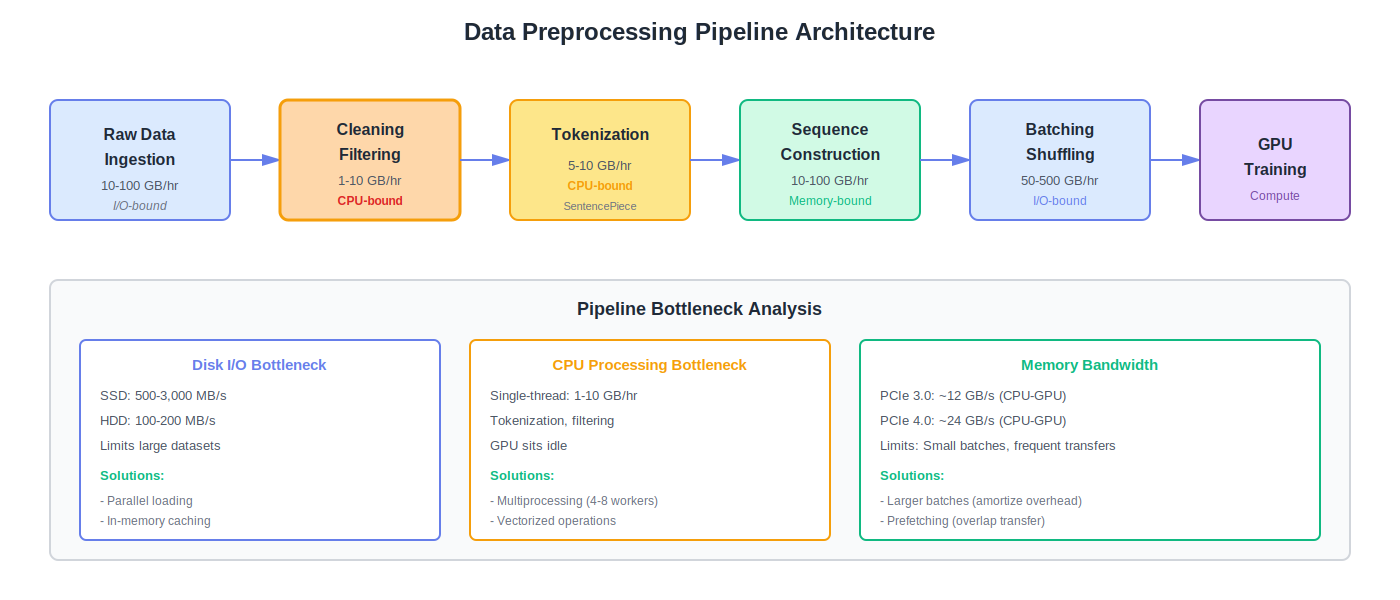
\includegraphics[width=0.95\textwidth]{chapters/diagrams/chapter08_data_pipeline_a1b2c3d4.pdf}
\caption{Data preprocessing pipeline architecture showing stages from raw data ingestion through batching. Bottlenecks typically occur at cleaning/filtering (CPU-bound) and disk I/O (storage-bound) stages.}
\label{fig:data_pipeline}
\end{figure}


\subsection{Pipeline Cost Analysis}

Pipeline infrastructure costs vary by scale and optimization level. Small-scale pipelines handling under 100 GB of data on a single machine require \$50-200 for SSD storage, with compute included in the training machine. Engineering effort of 1-2 weeks for setup dominates costs at \$10,000-20,000. This configuration suffices for initial development and small-scale experiments.

Medium-scale pipelines handling 100 GB to 10 TB of data across distributed systems require \$500-5,000 for distributed SSD or object storage. Compute needs expand to 4-16 preprocessing nodes. Engineering effort increases to 4-8 weeks for setup and optimization, totaling \$50,000-150,000. This scale supports regular training runs and moderate experimentation.

Large-scale pipelines exceeding 10 TB of data with production requirements demand \$5,000-50,000 for distributed object storage with redundancy. Dedicated preprocessing clusters handle continuous data flow. Engineering effort spans 3-6 months for development of robust, monitored pipelines, totaling \$200,000-1,000,000. This investment makes sense only for organizations running continuous training or large-scale experimentation programs.

The optimization decision hinges on training frequency and scale. For one-time training runs, simple pipelines suffice—the engineering cost of optimization exceeds the compute savings. For continuous training or large-scale experimentation, optimized pipelines provide substantial ROI. A pipeline that reduces training time by 30\% saves \$15,000 on a \$50,000 training run, justifying significant engineering investment after just a few runs.

\section{Data Augmentation and Synthetic Data}

\subsection{Augmentation Strategies}

Data augmentation artificially expands training datasets through transformations that preserve semantic meaning while introducing variation. This technique reduces data collection costs and improves model robustness by exposing the model to diverse phrasings and formulations of similar content.

Back-translation translates text to another language and back, introducing paraphrasing while preserving meaning. Using translation APIs costs \$0.001-0.01 per example, far less than human annotation. Effectiveness varies by task: low-resource tasks see 10-30\% accuracy improvement, while high-resource tasks see 5-10\% improvement. The technique works best for tasks where paraphrasing doesn't change labels, such as sentiment analysis or topic classification.

Synonym replacement substitutes words with synonyms from WordNet or embedding-based similarity. Computational cost is negligible—a few milliseconds per example. Effectiveness reaches 5-15\% improvement for classification tasks, though care must be taken to avoid changing meaning. The technique fails for tasks requiring precise wording, such as named entity recognition or question answering.

Random insertion, deletion, and swapping introduce noise that improves model robustness. These techniques cost nothing computationally and provide 3-8\% improvement on classification tasks. The approach works by forcing the model to focus on semantic content rather than specific word positions or exact phrasing. Effectiveness depends on noise level—too little provides minimal benefit, too much degrades training signal.

Contextual word replacement uses language models to generate contextually appropriate substitutions. This technique costs \$0.0001-0.001 per example using API-based language models, or runs locally at negligible cost with open-source models. Effectiveness reaches 10-20\% improvement for tasks requiring semantic understanding. The technique generates more natural variations than simple synonym replacement, though at higher computational cost.

\subsection{Synthetic Data Generation}

Synthetic data generation creates training examples programmatically, reducing or eliminating human annotation costs. This approach works best when the generation process can be validated and when synthetic examples closely match production distribution.

Template-based generation creates examples from predefined patterns. For structured tasks like form filling or database queries, templates can generate millions of valid examples at near-zero cost. A template for customer support queries might generate "I need help with [product] [issue]" with systematic variation of products and issues. This approach works when the task structure is well-defined and the template space covers production distribution adequately.

Rule-based generation applies domain rules to create valid examples. For code generation tasks, syntax rules ensure generated code is valid. For data extraction tasks, rules define valid entity relationships. The cost is primarily engineering time to develop and validate rules—typically 2-4 weeks for a comprehensive rule set. Once developed, generation costs are negligible. Effectiveness depends on rule coverage: comprehensive rules generate high-quality data, incomplete rules introduce systematic biases.

Model-based generation uses trained language models to generate examples. GPT-4 or similar models can generate training data at \$0.01-0.10 per example, still cheaper than human annotation at \$0.50-5.00 per example. Quality varies significantly: simple tasks yield 80-90\% usable examples, complex tasks yield 40-60\% usable examples. Human review remains necessary to filter low-quality generations, but the cost savings can reach 50-70\% compared to full human annotation.

The critical consideration for synthetic data is distribution match. Synthetic examples that differ systematically from production data degrade model performance despite high volume. Validation requires comparing synthetic and production distributions across multiple dimensions: vocabulary, syntax, semantic patterns, and edge cases. Mismatches indicate the need for generation process refinement or supplemental real data collection.

\subsection{Augmentation Economics}

Data augmentation economics follow a clear pattern: augmentation costs far less than original data collection, but provides diminishing returns. The first 2× data expansion through augmentation typically costs 5-10\% of original collection costs and provides 10-20\% accuracy improvement. The next 2× expansion costs similar amounts but provides only 5-10\% additional improvement. Beyond 4× expansion, returns diminish rapidly.

For a project with 10,000 labeled examples costing \$50,000 to collect, augmentation to 40,000 examples costs \$2,500-5,000 and might improve accuracy from 85\% to 92\%. Further augmentation to 160,000 examples costs another \$2,500-5,000 but might improve accuracy only to 94\%. The optimization question centers on whether the marginal accuracy improvement justifies the cost and whether collecting additional real data would provide better returns.

The strategic decision depends on data availability and task characteristics. When real data is scarce or expensive—medical imaging, specialized domains, rare events—aggressive augmentation makes sense. When real data is abundant and cheap—web text, common images, standard classification—minimal augmentation suffices, with resources better spent on data quality or model optimization.

\section{Training Monitoring and Evaluation}

\subsection{Monitoring Infrastructure}

Training monitoring tracks model convergence, identifies issues early, and enables informed intervention decisions. Effective monitoring prevents wasted compute from failed training runs and provides data for optimization decisions.

Loss curves track training and validation loss over time, providing the primary signal of training progress. Training loss should decrease steadily; plateaus indicate learning rate issues or optimization problems. Validation loss should track training loss initially, then diverge as the model begins overfitting. The gap between training and validation loss quantifies overfitting severity. Monitoring both curves enables early stopping—terminating training when validation loss stops improving—saving compute resources that would otherwise be wasted on overfitting.

Learning rate schedules require monitoring to ensure appropriate adjustment timing. Warmup periods at the start of training prevent instability from large initial updates. Decay schedules reduce learning rate as training progresses, enabling fine-grained optimization. Monitoring loss curves during schedule transitions identifies whether adjustments occur at appropriate times. Premature decay slows learning unnecessarily; delayed decay wastes compute on suboptimal updates.

Gradient statistics reveal optimization health. Gradient norms that grow unboundedly indicate instability requiring learning rate reduction or gradient clipping. Gradient norms that approach zero indicate vanishing gradients, suggesting architectural issues or learning rate problems. Monitoring gradient statistics enables early detection of training failures before they waste significant compute resources.

Resource utilization monitoring tracks GPU utilization, memory consumption, and data loading throughput. Low GPU utilization indicates data loading bottlenecks or inefficient batching. High memory consumption approaching limits suggests batch size reduction or gradient accumulation. Monitoring these metrics enables infrastructure optimization and prevents out-of-memory failures that waste training progress.

\begin{figure}[htbp]
\centering
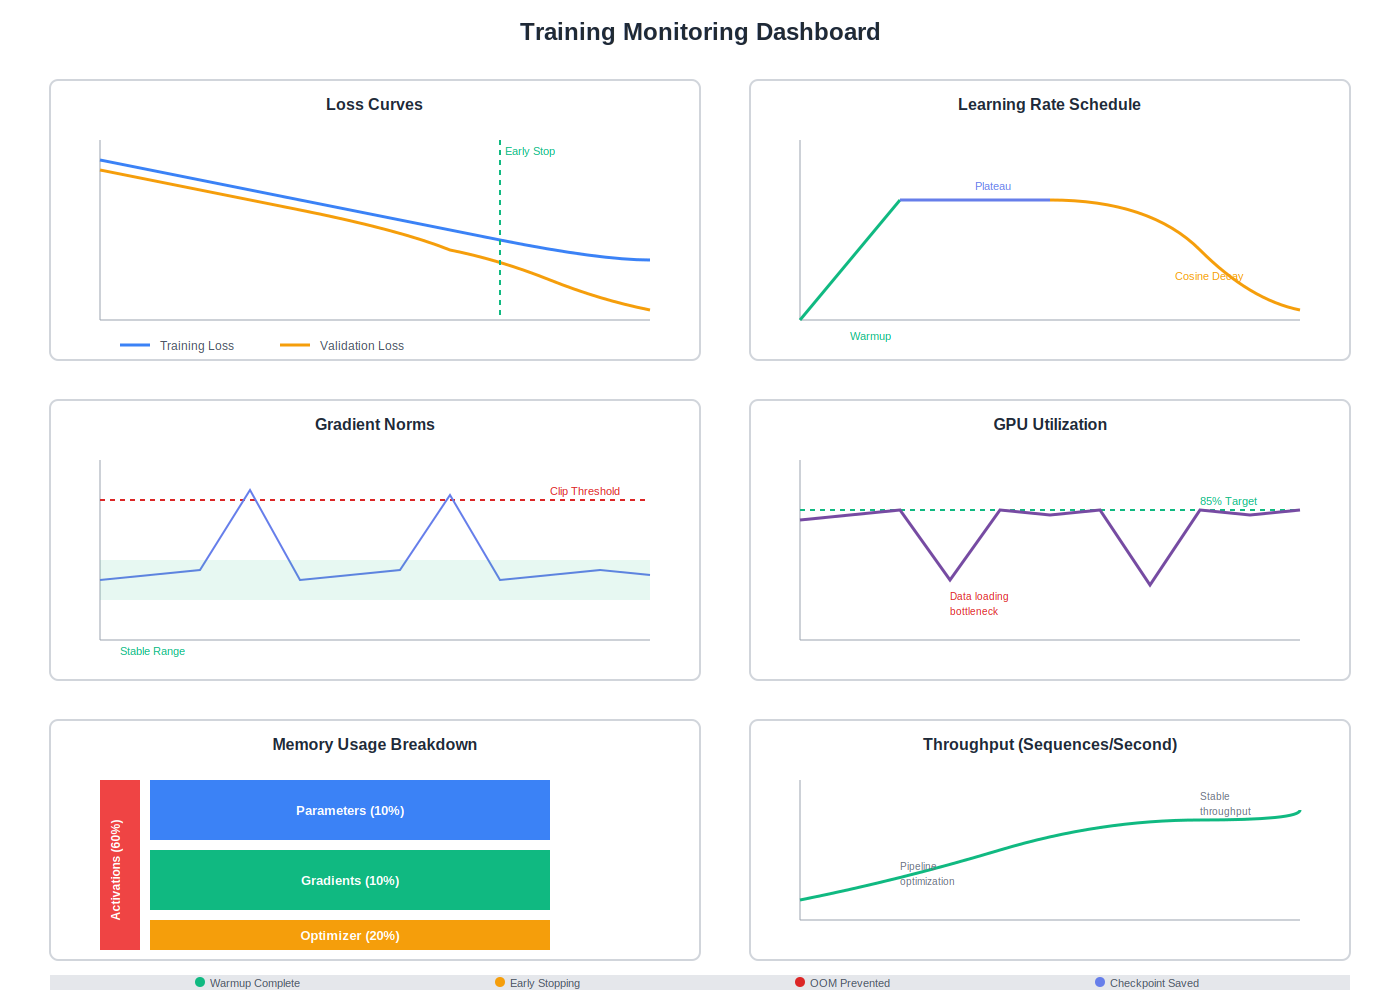
\includegraphics[width=0.95\textwidth]{chapters/diagrams/chapter08_monitoring_q7r8s9t0.pdf}
\caption{Training monitoring dashboard showing key metrics: loss curves with early stopping point, learning rate schedule phases, gradient norms with clipping threshold, GPU utilization with data loading spikes, memory breakdown by component, and throughput improvements over time. Comprehensive monitoring enables early issue detection and informed intervention decisions.}
\label{fig:monitoring_dashboard}
\end{figure}

\subsection{Evaluation Frameworks}

Evaluation frameworks measure model performance on held-out test data, providing unbiased estimates of production performance. The framework design determines whether evaluation results predict production success or mislead with optimistic estimates.

Test set construction requires careful attention to distribution match. Test data should represent production distribution across all relevant dimensions: input types, edge cases, and temporal variation. Systematic differences between test and production distributions lead to evaluation-production performance gaps that undermine deployment confidence. For time-series data, temporal splits prevent data leakage; for user-generated content, user-based splits prevent overfitting to specific users.

Metric selection should align with business objectives. Accuracy measures overall correctness but may hide performance issues on important subgroups. Precision and recall trade off false positives versus false negatives, with optimal balance depending on error costs. F1 score balances precision and recall but may not reflect business priorities. For imbalanced datasets, metrics like AUC-ROC or average precision provide more informative evaluation than raw accuracy.

Subgroup analysis identifies performance disparities across important segments. A model with 90\% overall accuracy might achieve 95\% on common cases but only 70\% on rare but important cases. Analyzing performance by input type, user segment, or edge case category reveals these disparities. Production deployment requires acceptable performance across all critical segments, not just high average performance.

Error analysis examines failure cases to identify systematic issues. Clustering errors by type—missing information, ambiguous inputs, edge cases—reveals whether failures are random or systematic. Systematic failures indicate training data gaps, architectural limitations, or preprocessing issues that can be addressed. Random failures may represent irreducible task difficulty. The distinction determines whether additional investment can improve performance or whether current performance represents a practical ceiling.

\begin{tcolorbox}[colback=red!5!white,colframe=red!75!black,title=\textbf{COMMON MISTAKES: Evaluation Pitfalls}]

\textbf{Data Leakage}: Test data that overlaps with training data produces optimistic performance estimates that don't generalize to production. This occurs through duplicate examples, temporal leakage in time-series data, or information leakage through preprocessing. Rigorous data splitting and validation prevents this issue.

\textbf{Metric Mismatch}: Optimizing for metrics that don't align with business objectives leads to models that perform well on benchmarks but poorly in production. A customer support model optimized for accuracy might achieve high scores by handling easy queries well while failing on difficult but important cases. Metric selection should reflect actual business priorities and error costs.

\textbf{Insufficient Test Coverage}: Test sets that don't represent production distribution lead to evaluation-production performance gaps. A model tested only on clean, well-formatted inputs may fail on noisy production data. Test sets should include edge cases, adversarial examples, and distribution shifts likely in production.

\end{tcolorbox}

\section{Hyperparameter Optimization}

\subsection{Optimization Strategies}

Hyperparameter optimization searches for configurations that maximize model performance. The search space includes learning rate, batch size, model architecture parameters, regularization strength, and optimizer settings. Effective optimization balances exploration of the search space against computational cost.

Grid search evaluates all combinations of predefined hyperparameter values. For three hyperparameters with five values each, this requires 125 training runs. The approach guarantees finding the best combination within the search space but becomes prohibitively expensive for large search spaces. Grid search works best for small search spaces with 2-3 hyperparameters and 3-5 values each, requiring 10-100 training runs.

Random search samples hyperparameter combinations randomly from defined ranges. This approach explores the search space more efficiently than grid search, often finding good configurations with fewer evaluations. For the same computational budget as grid search, random search typically finds better configurations by exploring more diverse combinations. The approach works well for medium search spaces with 4-6 hyperparameters, requiring 50-200 training runs to find near-optimal configurations.

Bayesian optimization builds a probabilistic model of the hyperparameter-performance relationship and uses this model to guide search toward promising regions. This approach requires fewer evaluations than random search—typically 20-50 training runs—but adds optimization overhead. The technique works best for expensive training runs where minimizing evaluations justifies the optimization complexity. Tools like Optuna and Ray Tune provide production-ready Bayesian optimization implementations.

Population-based training runs multiple training processes in parallel, periodically copying hyperparameters from high-performing runs to low-performing runs. This approach combines hyperparameter search with training, reducing total wall-clock time. The technique requires substantial parallel compute resources—typically 10-50 simultaneous training runs—but can find good configurations faster than sequential approaches. The method works best when parallel compute is available and training time is the primary constraint.

\begin{figure}[htbp]
\centering
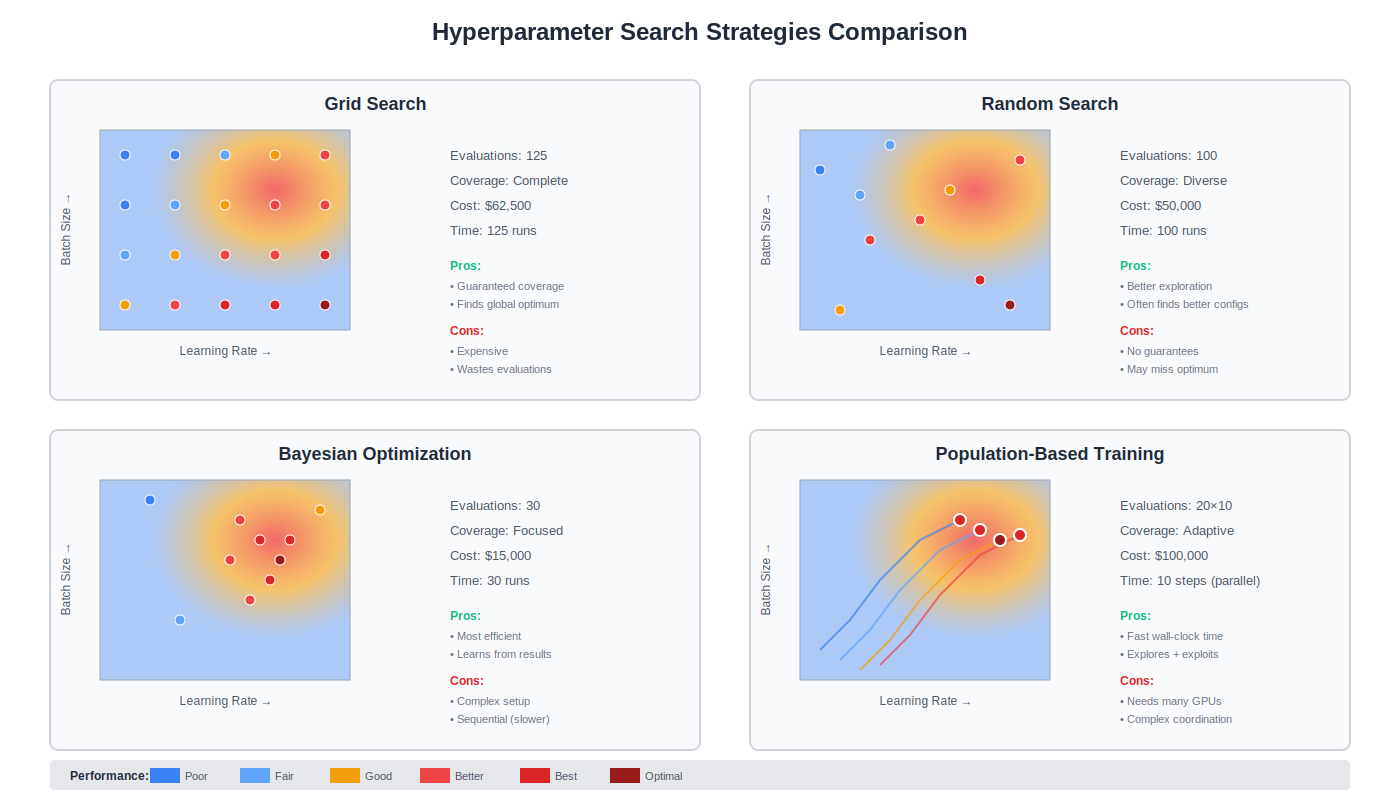
\includegraphics[width=0.95\textwidth]{chapters/diagrams/chapter08_hyperparameter_m3n4o5p6.pdf}
\caption{Hyperparameter search strategy comparison showing exploration patterns and efficiency trade-offs. Grid search provides complete coverage but wastes evaluations; random search explores more efficiently; Bayesian optimization focuses on promising regions; population-based training parallelizes search for faster wall-clock time.}
\label{fig:hyperparameter_search}
\end{figure}

\subsection{Optimization Economics}

Hyperparameter optimization costs scale with search space size and training cost per configuration. For BERT-base training costing \$500 per run, a 100-configuration random search costs \$50,000. This investment makes sense when the resulting model will be deployed at scale, where performance improvements translate to substantial operational savings or revenue increases.

The optimization strategy should match project economics. For research projects or one-time deployments, minimal optimization with 5-10 manual trials suffices. For production systems serving millions of requests, comprehensive optimization with 50-200 trials justifies its cost through improved performance. For continuous training pipelines, automated optimization infrastructure amortizes its development cost across multiple projects.

Early stopping and performance prediction reduce optimization costs by terminating unpromising configurations early. A configuration showing poor performance after 10\% of training is unlikely to become competitive by completion. Terminating such runs early saves 90\% of their compute cost. Across a 100-configuration search, early stopping might reduce total cost by 40-60\% by eliminating poor configurations quickly.

\section{Data Versioning and Reproducibility}

\subsection{Versioning Infrastructure}

Data versioning tracks dataset changes over time, enabling reproducibility and debugging. As training data evolves through collection, cleaning, and augmentation, versioning provides an audit trail of what data produced which model performance.

Dataset versioning systems like DVC (Data Version Control) or Pachyderm track dataset changes using content-addressable storage. Each dataset version receives a unique identifier based on its content. Models trained on specific dataset versions can be traced back to exact training data, enabling reproducibility and debugging. The storage cost depends on dataset size and change frequency: for 100 GB datasets with monthly updates, storage costs run \$50-200 monthly for cloud object storage with versioning.

Preprocessing pipeline versioning tracks code changes that transform raw data into training data. A bug in preprocessing can corrupt training data, degrading model performance in ways difficult to diagnose without versioning. Git-based versioning of preprocessing code combined with dataset versioning provides complete reproducibility. The engineering cost is minimal—standard version control practices—but the debugging value is substantial when issues arise.

Experiment tracking systems like Weights & Biases, MLflow, or Neptune link models to dataset versions, hyperparameters, and training code. This linkage enables reproducing any training run exactly and understanding what changed between runs. For teams running dozens or hundreds of experiments, this tracking infrastructure is essential for maintaining productivity and avoiding duplicate work.

\subsection{Reproducibility Practices}

Reproducibility requires controlling all sources of randomness and variation. Random seeds for data shuffling, weight initialization, and dropout must be fixed and recorded. Hardware differences—GPU models, driver versions, library versions—can affect results, requiring documentation. The goal is not perfect bit-level reproducibility, which is often impractical, but rather the ability to reproduce results within acceptable tolerance.

Containerization using Docker or similar tools captures the complete software environment, including library versions, system dependencies, and configuration. A containerized training environment can be archived and rerun months or years later, producing comparable results. The storage cost is minimal—typically a few GB per container—while the reproducibility value is substantial for debugging and auditing.

Documentation practices complement technical versioning. Training run documentation should include dataset version, preprocessing pipeline version, hyperparameters, training duration, final performance metrics, and any anomalies observed. This documentation enables future debugging and provides context for comparing runs. The time cost is 10-15 minutes per training run, negligible compared to training time but valuable for long-term project management.

\section{Key Insights}

\textbf{Data Quality Dominates Architecture}: Model performance depends more on training data quality than architectural sophistication. A well-designed model trained on poor data underperforms a simpler model trained on high-quality data. Data quality investment—annotation accuracy, coverage, consistency—provides better returns than architectural complexity for most applications.

\textbf{Pipeline Bottlenecks Waste Compute}: Data loading bottlenecks cause GPU idle time, wasting expensive compute resources. A GPU capable of 1,000 sequences per second achieves only 100 sequences per second if data loading provides only 100 sequences per second. Pipeline optimization—parallel loading, prefetching, caching—directly improves training efficiency and reduces costs.

\textbf{Augmentation Shows Diminishing Returns}: The first 2× data expansion through augmentation provides 10-20\% accuracy improvement at 5-10\% of original collection cost. Further expansion provides diminishing returns. Beyond 4× expansion, collecting additional real data typically provides better returns than additional augmentation.

\textbf{Monitoring Prevents Wasted Compute}: Early detection of training failures through monitoring prevents wasted compute on failed runs. Loss curves, gradient statistics, and resource utilization monitoring enable intervention before significant resources are consumed. For expensive training runs, monitoring infrastructure pays for itself by preventing a single failed run.

\textbf{Hyperparameter Optimization Costs Scale Rapidly}: Comprehensive hyperparameter search with 100+ configurations can cost 100× a single training run. This investment makes sense for production deployments at scale but not for research projects or one-time applications. Optimization strategy should match deployment scale and expected operational lifetime.

\textbf{Versioning Enables Debugging}: Data and code versioning provide an audit trail that enables reproducing results and debugging performance issues. When model performance degrades, versioning enables identifying what changed—data, preprocessing, hyperparameters, or code. The infrastructure cost is minimal compared to the debugging value when issues arise.

The next chapter examines team building and organizational structure for AI projects, focusing on role definitions, skill requirements, and collaboration patterns that enable effective execution.

